\documentclass{beamer}
%%%%%%%%%%%%%%%%%%%%%%%%%%%%%%%%%%%%%%%%%%%%%%%%%%%%%%%%%%%%%%%%%%%%%%%%%%%%
\usepackage{bm}
\usepackage{amsmath}
\usepackage{amssymb}
%\usepackage{microtype}
\usepackage{booktabs} % \toprule, \midrule, \bottomrule
/Users/seth/Documents/Compositions/SRJinclude.tex
\newcommand{\Dtens}{\mat{D}}
\definecolor{lightgray}{gray}{0.85}
\newcommand{\notebox}[1]{\hspace{.1\columnwidth}\colorbox{lightgray}{\parbox{0.8\columnwidth}{\small
#1}}}
\newcommand{\epsiloncolor}[1]{\textcolor{blue}{#1}}
%%%%%%%%%%%%%%%%%%%%%%%%%%%%%%%%%%%%%%%%%%%%%%%%%%%%%%%%%%%%%%%%%%%%%%%%%%%%

\usetheme{AnnArbor}
\usecolortheme{seahorse}
\usecolortheme{orchid}
\usefonttheme[onlymath]{serif}
\setbeamercolor*{frametitle}{use=structure,bg=structure.fg!20!white}
\setbeamercolor*{frametitle right}{use=structure,bg=structure.fg!20!white}
\setbeamertemplate{navigation symbols}{\insertframenavigationsymbol}
\setbeamertemplate{caption}[numbered]

\title[Thesis Prospectus]%
{A Physics-Based Anisotropic Diffusion Method for Thermal Radiative
Transfer}
%\subtitle{}

\author[SRJ]{Seth~R.~Johnson}

\institute[UMich]{
University of Michigan, Ann Arbor
}
\date[11/3/2010]{November 3, 2010}

%\AtBeginSection[]
%{
%\begin{frame}
%  \frametitle{Outline}
%  \tableofcontents[currentsection]
%\end{frame}
%}
%
\hypersetup{colorlinks=true,linkcolor=black}

% only show section headings in table of contents
\setcounter{tocdepth}{1}

%use symbols for footnote
\renewcommand{\thefootnote}{\fnsymbol{footnote}}

\begin{document}
%%%%%%%%%%%%%%%%%%%%%%%%%%%%%%%%%%%%%%%%%%%%%%%%%%%%%%%%%%%%%%%%%%%%%%%%%%%%

\begin{frame}
\titlepage
\begin{center}
  \includegraphics[width=0.2\textwidth]{../figures/umlogo}
\end{center}
\end{frame}

%%%%%%%%%%%%%%%%%%%%%%%%%%%%%%%%%%%%%%%%%%%%%%%%%%%%%%%%%%%%%%%%%%%%%%%%%%%%
\section{Introduction}
%%%%%%%%%%%%%%%%%%%%%%%%%%%%%%%%%%%%%%%%
\begin{frame}
  \frametitle{Thermal radiative transfer}
  \begin{itemize}
    \item TRT is the dominant heat transfer process in very hot materials
    \item High-energy photons are emitted $\propto T^4$ by hot material and
      absorbed by cold
    \item Cold material heats up and becomes relatively transparent (smaller
      $\sigma$)
  \end{itemize}

  Applications in high energy density physics:
  \begin{itemize}
    \item Stellar astrophysics, strategic astrophysics
    \item Inertial confinement fusion
    \item CRASH (Center for RAdiative Shock Hydrodynamics) program: ``Assessment
          of Predictive Capability''
  \end{itemize}
  Difficulties in solving:
  \begin{itemize}
    \item High dimensionality of solution phase space $(\vec{x}, \vec{\Omega},
      h\nu, t)$
    \item Highly nonlinear coupled partial differential equations for radiation
      field $I(\vec{x}, \vec{\Omega}, h\nu, t)$ and material energy $U_m(\vec{x}, t)$
  \end{itemize}
\end{frame}
%%%%%%%%%%%%%%%%%%%%%%%%%%%%%%%%%%%%%%%%
\begin{frame}
  \frametitle{Motivation}
\begin{center}
  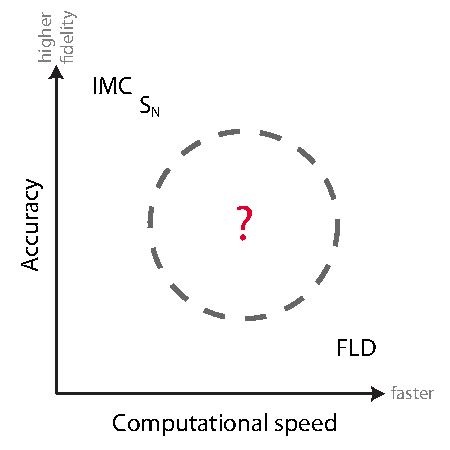
\includegraphics[width=3in]{../figures/fidelity}
\end{center}
% also, storage requirements
\end{frame}
%%%%%%%%%%%%%%%%%%%%%%%%%%%%%%%%%%%%%%%%
\begin{frame}
  \frametitle{Previous work}
  \begin{itemize}
    \item Steady-state VHTR-like problem with analytically calculated
      coefficients \cite{Lar2009c}
    \item Non-local tensor diffusion \cite{Mor2007} for steady-state
      radiative transfer, no further development or
      analysis in literature
  \end{itemize}
\end{frame}
%%%%%%%%%%%%%%%%%%%%%%%%%%%%%%%%%%%%%%%%%%%%%%%%%%%%%%%%%%%%%%%%%%%%%%%%%%%%
\section{Theory}
%%%%%%%%%%%%%%%%%%%%%%%%%%%%%%%%%%%%%%%%
\begin{frame}
  \frametitle{Summary in advance}
  \begin{enumerate}
    \item Make assumptions about weakness of derivatives and moments of angular
      flux $I(\vec{x}, \vec{\Omega}, t)$. % non-rigorous $O(1)$, $O(\epsilon)$
    \item Substitute the particle conservation equation (zeroth moment of
      Boltzmann equation) into the integral equation for time-dependent
      intensity.
    \item Apply Taylor series to non-local $\phi$ to get an approximate
      expression for $I(\vec{x}, \vec{\Omega}, t)$ as a function of
      $\phi(\vec{x}, t)$ and other problem-dependent quantities.
      Discard $O(\epsilon^2)$ and higher terms.
    \item Take first moment of this approximate $I$ to get
      $\vec{F}(\vec{x}, t)$.
    \item Apply semi-implicit approximation to TRT equations
  \end{enumerate}
\end{frame}

\subsection{Anisotropic diffusion derivation}
%%%%%%%%%%%%%%%%%%%%%%%%%%%%%%%%%%%%%%%%
\begin{frame}
  Gray Boltzmann transport equation:
  \begin{multline} \label{eq:fullGrayTransport2}
  \frac{1}{c} \pder{I}{t}(\vec{x}, \vec{\Omega}, t)
  + \vec{\Omega} \vd \del I(\vec{x}, \vec{\Omega}, t) +
 \sigma(\vec{x}, t) I(\vec{x}, \vec{\Omega}, t)
  \\= \frac{\sigma(\vec{x}, t) a c [T(\vec{x},t)]^4}{4\pi} 
  + \frac{c Q(\vec{x},t)}{4\pi}
  %\,, \qquad \vec{x} \in V, \ \vec{\Omega} \in 4\pi, \ t >= 0.
  \end{multline}
  Radiation energy conservation by integrating over angles $\int_{4\pi} (\cdot) \ud
  \Omega$:
  \begin{equation} \label{eq:grayTransportZeroth}
  \frac{1}{c} \pder{\phi}{t}(\vec{x}, t)
  +\del \vd \vec{F}(\vec{x}, t) +
 \sigma(\vec{x}, t) \phi(\vec{x}, t)
  = \sigma(\vec{x}, t) a c [T(\vec{x},t)]^4
  + c Q(\vec{x},t)
  \end{equation}

  \begin{block}{Asymptotic importance ansatz}
    \begin{align*}
  I &= O(\epsiloncolor{1}), &
  \sigma &= O(\epsiloncolor{1}), \\
  \del I &= O(\epsiloncolor{\epsilon}), &
  \frac1c\pder{I}{t} &= O(\epsiloncolor{\epsilon}), &
  \int_{4\pi} \vec{\Omega} I\ud \Omega &= O(\epsiloncolor{\epsilon}).
    \end{align*}
  \end{block}
\end{frame}
%%%%%%%%%%%%%%%%%%%%%%%%%%%%%%%%%%%%%%%%
\begin{frame}
  Integral time-dependent transport equation \cite{Pri2010}, neglecting
  boundary and initial conditions:
  \begin{equation} \label{eq:integralAngularFluxShortened}
    I(\vec{x}, \vec{\Omega}, t)
    = \int_{0}^{\infty}
    \eexp^{ -\tau(\vec{x}, \vec{x} - s \vec{\Omega}, \vec{\Omega}, t)}
    \left[ \frac{\sigma a c T^4}{4\pi} + \frac{c Q}{4\pi} \right]_{(\vec{x} - s
    \vec{\Omega}, t-s/c)} \ud s
  \end{equation}
  where the optical thickness from $(\vec{x},t)$ to the boundary along
  $\vec{\Omega}$ is
  \begin{equation} \label{eq:integralTrtTauDefinition}
    \tau(\vec{x}, \vec{x}', \vec{\Omega}, t) = \int_{0}^{\norm{\vec{x} -
    \vec{x}'}} \sigma(\vec{x}-s'\vec{\Omega}, t-s'/c) \ud s' \,.
  \end{equation}
  Substituting left hand side of conservation
  equation~\eqref{eq:grayTransportZeroth}:
  \begin{align}
    I(\vec{x}, \vec{\Omega}, t)
    &= \frac{1}{4\pi} \int_{0}^{\infty}
    \eexp^{ -\tau(\vec{x}, \vec{x} - s \vec{\Omega}, \vec{\Omega}, t)}
    \left[ \sigma a c T^4 + cQ \right]_{(\vec{x} - s \vec{\Omega}, t-s/c)} \ud s
    \nonumber\\
    &= \frac{1}{4\pi}\int_{0}^{\infty}
    \eexp^{ -\tau(\vec{x}, \vec{x} - s \vec{\Omega}, \vec{\Omega}, t)}
    \bigg[
    \underbrace{\sigma \phi\vphantom{\frac1c}}_{O(1)}
    + \underbrace{\frac{1}{c} \pder{\phi}{t}}_{O(\epsilon)}
    + \underbrace{\del \vd \vec{F}\vphantom{\frac1c}}_{O(\epsilon^2)}
    \bigg]_{(\vec{x} - s \vec{\Omega}, t-s/c)} \ud s
    \label{eq:integralTrtRhs}
  \end{align}
\end{frame}
%%%%%%%%%%%%%%%%%%%%%%%%%%%%%%%%%%%%%%%%
\begin{frame}%{The first component of $I$}
%\begin{align*}
%  \lefteqn{\eexp^{ -\tau(\vec{x}, \vec{x} - s \vec{\Omega}, \vec{\Omega}, t)}
%  \sigma(\vec{x} - s \vec{\Omega}, t-s/c)}\qquad&
%  \\
%  &= \sigma(\vec{x} - s \vec{\Omega}, t-s/c) \expp{ -\int_{0}^{s}
%  \sigma(\vec{x}-s'\vec{\Omega}, t-s'/c) \ud s'}
%  \\
%  &= -\oder{}{s}
%    \expp{ -\int_{0}^{s} \sigma(\vec{x}-s'\vec{\Omega}, t-s'/c) \ud s'}
%\end{align*}
\begin{align*}
\lefteqn{\frac{1}{4\pi}\int_{0}^{\infty} \eexp^{ -\int_{0}^{s}
  \sigma(\vec{x}-s'\vec{\Omega}, t-s'/c) \ud s'} \sigma(\vec{x} - s \vec{\Omega}, t-s/c)
\phi(\vec{x} - s \vec{\Omega}, t-s/c) \ud s}\qquad&
\\ 
\intertext{Fundamental theorem of calculus:}
&=\frac{1}{4\pi}\int_{0}^{\infty} \left( - \oder{}{s} \eexp^{ -\int_{0}^{s}
  \sigma(\vec{x}-s'\vec{\Omega}, t-s'/c) \ud s'}\right)
\phi(\vec{x} - s \vec{\Omega}, t-s/c) \ud s
\\
\intertext{Integration by parts with $u=\phi(\vec{x} - s \vec{\Omega}, t-s/c)$
and $\ud v = \oder{}{s} \eexp^{-\tau} \ud s$:}
    \begin{split}
  &=-\frac{1}{4\pi} \bigg[ 
\eexp^{- \int_{0}^{s} \sigma(\vec{x}-s'\vec{\Omega}, t-s'/c) \ud s'} 
\phi(\vec{x} - s \vec{\Omega}, t-s/c) \bigg|_{0}^{\infty}
\\
&\qquad\qquad- \int_{0}^{\infty} \eexp^{- \int_{0}^{s} \sigma(\vec{x}-s'\vec{\Omega}, t-s'/c) \ud s'}
\oder{}{s} \phi(\vec{x} - s \vec{\Omega}, t-s/c)
\ud s
  \bigg]
    \end{split}
  \\
  &=-\frac{1}{4\pi} \bigg[ 
0 -  
\eexp^0 \phi(\vec{x}, t)
- \int_{0}^{\infty} \eexp^{-\tau(\vec{x}, \vec{x} - s \vec{\Omega}, \vec{\Omega}, t)}
\oder{}{s} \phi(\vec{x} - s \vec{\Omega}, t-s/c)
\ud s
  \bigg]
%  \\
% &=\frac{1}{4\pi}\phi(\vec{x}, t)
%+ \frac{1}{4\pi}\ \int_{0}^{\infty} \eexp^{-\tau(\vec{x}, \vec{x} - s \vec{\Omega}, \vec{\Omega}, t)}
%\oder{}{s} \phi(\vec{x} - s \vec{\Omega}, t-s/c)
%\ud s
 \\
    %\begin{split}
 &=\frac{1}{4\pi}\phi(\vec{x}, t)
% \\
%&\qquad
+ \frac{1}{4\pi}\ \int_{0}^{\infty} \eexp^{-\tau}
\left[ -\vec{\Omega} \vd \del - \pder{}{t} \right] \phi(\vec{x} - s \vec{\Omega}, t-s/c)
\ud s
%    \end{split}
%  \\
%  &= O(\epsiloncolor{1}) + O(\epsiloncolor{\epsilon})
\end{align*}
%(assuming $\phi\to 0$ as $\norm{\vec{x}}\to \infty$)
\end{frame}
%%%%%%%%%%%%%%%%%%%%%%%%%%%%%%%%%%%%%%%%
\begin{frame}{Approximate using Taylor series}
  Taylor series expansion of nonlocal unknown $\phi$ in space and time:
  \begin{align*}
  \phi(\vec{x} - s \vec{\Omega}, t-s/c)
  &\sim
  \phi(\vec{x}, t) - s \vec{\Omega} \vd \del \phi(\vec{x}, t)
  - s\frac{1}{c} \pder{\phi}{t}(\vec{x}, t) + \cdots
  \\
  &= \phi(\vec{x}, t) - s \left[ \vec{\Omega} \vd \del
  + \frac{1}{c} \pder{}{t} \right] \phi(\vec{x}, t) + \cdots
  \\
  &= O(\epsiloncolor{1}) +
  O(\epsiloncolor{\epsilon}) + \cdots
  \end{align*}

  Taylor series in time for $\sigma$ embedded in optical thickness $\tau$:
\begin{align*}
  \sigma(\vec{x} - s \vec{\Omega}, t-s/c)
  &\sim
  \sigma(\vec{x} - s \vec{\Omega}, t)
  - s\frac{1}{c} \pder{\sigma}{t}(\vec{x} - s \vec{\Omega}, t) + \cdots
  \\
  &= O(\epsiloncolor{1}) + O(\epsiloncolor{\epsilon^{(?)}}) + \cdots
\end{align*}
Keep only the leading order terms.
%  Derivative along streaming direction:
%  \begin{align*}
%    \oder{}{s} f(\vec{x} - s \vec{\Omega}, t-s/v)
%    &=  \oder{}{s} f(x_i - s \Omega_i, t-s/v)
%    = \oder{}{s} f(x_1',x_2',x_3',t')
%    \\
%    &= \sum_{i=1}^{3}
%    \pder{x_i'}{s}\pder{x_i}{x_i'} \pder{f}{x_i}
%    + \pder{t'}{s}\pder{t}{t'} \pder{f}{t}
%    \\
%    &= \sum_{i=1}^{3} [- \Omega_i][1]\pder{f}{x_i} 
%    + \left( -\frac{1}{v} \right)  \pder{f}{t}
%    \\
%    &= \left[ -\vec{\Omega} \vd \del f - \pder{f}{t} \right]_{(\vec{x} - s
%    \vec{\Omega}, t-s/v)}
%  \end{align*}
\end{frame}
%%%%%%%%%%%%%%%%%%%%%%%%%%%%%%%%%%%%%%%%
\begin{frame}
 The expansion in $\phi$ allows it to be moved outside the integral, and the
 expansion in $\sigma$ obviates the storage of all prior $\sigma$:
\begin{multline*}
  \int_{0}^{\infty} \eexp^{- \int_{0}^{s} \sigma(\vec{x}-s'\vec{\Omega}, t-s'/c) \ud s'}
\left[ -\vec{\Omega} \vd \del - \pder{}{t} \right] \phi(\vec{x} - s \vec{\Omega}, t-s/c)
\ud s
\\
\sim \int_{0}^{\infty} \eexp^{- \int_{0}^{s} \sigma(\vec{x}-s'\vec{\Omega}, t)
\ud s'} \ud s
\left[ -\vec{\Omega} \vd \del - \pder{}{t} \right] \phi(\vec{x}, t)
\end{multline*}
Therefore the $\sigma\phi$ component of $I$ is approximated as
\begin{multline*}
  \frac{1}{4\pi}\int_{0}^{\infty} \eexp^{ -\tau(\vec{x}, \vec{x} - s
  \vec{\Omega}, \vec{\Omega}, t)} \sigma(\vec{x} - s \vec{\Omega}, t-s/c)
  \phi(\vec{x} - s \vec{\Omega}, t-s/c) \ud s
  \\
  \sim 
  \frac{1}{4\pi}\underbrace{\phi(\vec{x}, t)}_{O(1)}
  + \frac{1}{4\pi}\int_{0}^{\infty} \eexp^{- \int_{0}^{s} \sigma(\vec{x}-s'\vec{\Omega}, t)
\ud s'} \ud s
\underbrace{\left[ -\vec{\Omega} \vd \del - \pder{}{t} \right]}_{O(\epsilon)} \phi(\vec{x}, t)\,.
\end{multline*}
\end{frame}
%%%%%%%%%%%%%%%%%%%%%%%%%%%%%%%%%%%%%%%%
\begin{frame}
  Next term in Eq.~\eqref{eq:integralTrtRhs}: apply the same Taylor series to
  $\sigma$ and $\phi$, discarding $O(\epsilon^2)$ and higher terms:
\begin{multline*}
  \frac{1}{4\pi}\int_{0}^{\infty} \eexp^{ -\tau(\vec{x}, \vec{x} - s
  \vec{\Omega}, \vec{\Omega}, t)}
  \frac{1}{c} \pder{}{t}\phi(\vec{x} - s \vec{\Omega}, t-s/c) \ud s
 \\
 \sim 
  \frac{1}{4\pi}\int_{0}^{\infty} \eexp^{- \int_{0}^{s} \sigma(\vec{x}-s'\vec{\Omega}, t)
  \ud s'} \ud s
  \underbrace{\frac{1}{c} \pder{}{t}}_{O(\epsilon)}\phi(\vec{x}, t)\,.
\end{multline*}
This cancels the time derivative term from the $\sigma\phi$ component!

Third term in Eq.~\eqref{eq:integralTrtRhs},
  \begin{equation*}
    \frac{1}{4\pi}\int_{0}^{\infty} \eexp^{ -\tau(\vec{x}, \vec{x} - s
    \vec{\Omega}, \vec{\Omega}, t)}
    \del \vd \vec{F}(\vec{x} - s \vec{\Omega}, t-s/c) \ud s\,,
  \end{equation*}
is $O(\epsiloncolor{\epsilon^2})$, so neglect it.

Result: 
\begin{equation} \label{eq:anisotropicIntensity}
  I(\vec{x}, \vec{\Omega}, t) \approx
  \frac{1}{4\pi}\phi(\vec{x}, t) - \left[ \int_{0}^{\infty} \frac{1}{4\pi}
  \eexp^{- \int_{0}^{s} \sigma(\vec{x}-s'\vec{\Omega}, t)
  \ud s'} \ud s\right]
\vec{\Omega} \vd \del \phi(\vec{x}, t)
\end{equation}
\end{frame}

%%%%%%%%%%%%%%%%%%%%%%%%%%%%%%%%%%%%%%%%
\begin{frame}{Looks like Fick's law}
  Take the first angular moment of Eq.~\eqref{eq:anisotropicIntensity} to find
  the radiation flux:
\begin{align*}
  \vec{F}(\vec{x}, t) &= \int_{4\pi} \vec{\Omega} I(\vec{x}, \vec{\Omega}, t) \ud \Omega
  \\
  &=
  \frac{1}{4\pi}\phi(\vec{x}, t) \int_{4\pi} \vec{\Omega} \ud \Omega
  \\
  &\qquad-  \int_{4\pi} \vec{\Omega} \left[ \int_{0}^{\infty} \frac{1}{4\pi}
  \eexp^{- \int_{0}^{s} \sigma(\vec{x}-s'\vec{\Omega}, t)
  \ud s'} \ud s\right]
\vec{\Omega}  \ud \Omega \vd \del \phi(\vec{x}, t)
\\
&= - \Dtens(\vec{x},t) \vd \del \phi(\vec{x}, t)
\end{align*}
where $\Dtens$ is the second angular moment of the solution $f$ to the
``steady-state'' transport equation
\begin{equation} \label{eq:dcoeffTransportEquation}
  \vec{\Omega}\vd \del f(\vec{x},t) + \sigma(\vec{x},t) f(\vec{x},t) =
  \frac{1}{4\pi}\,.
\end{equation}
\end{frame}

\subsection{Anisotropic diffusion discussion}
%%%%%%%%%%%%%%%%%%%%%%%%%%%%%%%%%%%%%%%%
\begin{frame}
  \frametitle{Properties of anisotropic diffusion}

  The diffusion tensor $\Dtens(\vec{x},t)$: 
  \begin{itemize}
    \item Results from consistent approximations to the transport equation
      using physical coefficients
    \item Reduces to $\mat{I}/3\sigma$ for infinite homogeneous
      medium, which gives standard diffusion solution
    \item Has a smaller magnitude across a channel than along it
    \item Does not ``blow up'' in void regions
    \item Is continuous in $\vec{x}$, so the anisotropic solution $\phi$
      has continuous first derivatives
  \end{itemize}
\end{frame}

%%%%%%%%%%%%%%%%%%%%%%%%%%%%%%%%%%%%%%%%
\begin{frame}
  \begin{equation*}
    \vec{\Omega}\vd \del f + \sigma f = \frac{1}{4\pi}
  \end{equation*}

  The transport problem used to calculate $\Dtens$:
  \begin{itemize}
    \item Takes only one transport sweep to solve, since it is the description
      of a purely absorbing medium
    \item Only needs to be calculated once if $\sigma$ is constant in time
    \item Requires no storage of the angular flux, just accumulation of second
      moment, $D_{ij} = \int_{4\pi} \Omega_i \Omega_j f \ud \Omega$
  \end{itemize}
\end{frame}

%%%%%%%%%%%%%%%%%%%%%%%%%%%%%%%%%%%%%%%%%%%%%%%%%%%%%%%%%%%%%%%%%%%%%%%%%%%%
\subsection{Semi-implicit radiative transfer}
%%%%%%%%%%%%%%%%%%%%%%%%%%%%%%%%%%%%%%%%
\begin{frame}
  \frametitle{Thermal radiative transfer equations}
Zeroth moment of radiative transfer equation:
\begin{equation*}
  \frac{1}{c} \pder{\phi}{t}
  + \del \vd \vec{F} + \textcolor{red}{\sigma} \phi
  = \textcolor{red}{\sigma} ac\textcolor{red}{T^4}
  + c Q
\end{equation*}
Material energy balance equation:
\begin{equation*}
  \frac{1}{\textcolor{red}{c_v}}\pder{T}{t} = \textcolor{red}{\sigma} \phi -
  \textcolor{red}{\sigma} ac\textcolor{red}{T^4}
\end{equation*}

Semi-implicit discretization freezes $c_v/T^3$ and $\sigma$ at the initial time
value $t^n$ explicitly and treats $\vec{F}$ and $\phi$ implicitly. Some
manipulation gives a linear transport equation (with ``effective scattering''
that emulates photon absorption and re\"emission) over the time step, and an
equation to update the new material temperature.
%\notebox{\textcolor{red}{Red} quantities are temperature-dependent and couple
%the material energy to the radiation field.}
%
%Let equilibrium material radiation energy density be $U_r(T) \equiv aT^4$,
%material energy density be $U_m(T) \equiv \int_{0}^{T} c_v(T') \ud T'$, and
%\begin{equation*}
%  \beta(T) \equiv \pder{U_r}{U_m} 
%  = \pder{U_r}{T} \Bigg/ \pder{U_m}{T}
%  = \frac{4 a T^3}{c_v(T)} \,.
%\end{equation*}
\end{frame}

%%%%%%%%%%%%%%%%%%%%%%%%%%%%%%%%%%%%%%%%%%%%%%%%%%%%%%%%%%%%%%%%%%%%%%%%%%%%
\section{Results}
%%%%%%%%%%%%%%%%%%%%%%%%%%%%%%%%%%%%%%%%
\begin{frame}{Compared methods}
\begin{itemize}
  \item Implicit Monte Carlo \cite{Fle1971} (implemented with variance
    reduction methods), $10^6$ particles in each time step
  \item Flux-limited diffusion with Larsen limiter \cite{Ols2000}, with
    semi-implicit treatment of diffusion coefficient and radiation:
    \begin{equation*}
      \vec{F}^{n+1} = - D^{n} \del \phi^{n+1}  = -\left[ (3\sigma^{n})^2
      + \left( \frac{\norm{\del \phi^{n}}}{\phi^{n}}  \right)^2 \right]^{-1/2}
      \del \phi^{n+1}
    \end{equation*}
  \item Standard diffusion, with semi-implicit treatment of nonlinearities:
    \begin{equation*}
      \vec{F}^{n+1} = - D^{n} \del \phi^{n+1} 
      = -\frac{1}{3\sigma^{n}} \del \phi^{n+1}
    \end{equation*}
  \item Anisotropic diffusion, with 16 \SN{} quadrature angles per quadrant used
    to calculate $\Dtens$, with semi-implicit treatment of nonlinearities:
    \begin{equation*}
      \vec{F}^{n+1} = -\Dtens^{n}\vd \del \phi^{n+1} 
    \end{equation*}
\end{itemize}
\end{frame}

%%%%%%%%%%%%%%%%%%%%%%%%%%%%%%%%%%%%%%%%
\begin{frame}
  \frametitle{Summary of AD approximations}
  \begin{block}{Thermal radiative transfer equations}
    \begin{itemize}
      \item Assume weak gradients and angular moments for $I$
      \item Neglect boundary and initial conditions
      \item Semi-implicit approximation for the nonlinearities
    \end{itemize}
  \end{block}
  \begin{columns}[t]
    \begin{column}{.48\textwidth}
  \begin{block}{AD equation}
    \begin{itemize}
      \item Cell-centered finite difference spatial approximation
      \item Discard $D^{xy}$ and $D^{yx}$
    \end{itemize}
  \end{block}
    \end{column}
    \begin{column}{.48\textwidth}
  \begin{block}{$\Dtens$ transport equation}
    \begin{itemize}
      \item Discrete ordinates angular approximation
      \item Diamond difference spatial approximation (16 azimuthal ordinates
        per quadrant)
    \end{itemize}
  \end{block}
    \end{column}
  \end{columns}
\end{frame}

%%%%%%%%%%%%%%%%%%%%%%%%%%%%%%%%%%%%%%%%%%%%%%%%%%%%%%%%%%%%%%%%%%%%%%%%%%%%
\subsection{Test problem}
%%%%%%%%%%%%%%%%%%%%%%%%%%%%%%%%%%%%%%%%
\begin{frame}{Problem description}
  \begin{columns}[t]
    \begin{column}{.48\textwidth}
      Flatland geometry!

      Uniform spatial grid: $\Delta_x=0.1$
      
      Piecewise linear time grid: $\Delta_t=0.1$ for $t \ge 1$

      Reflecting bndy on left, others vacuum
    \end{column}
    \begin{column}{.48\textwidth}
      \textcolor[rgb]{0,0,1}{\textbf{Source}}: $c_v=0.5$, $\sigma=0.5$;
      $Q=1$ for $0 \le t \le 1$, $Q=0$ for $t > 1$.

      \textcolor[rgb]{0.1,0.9,0.1}{\textbf{Channel}}: $c_v=0.1$,
      $\sigma=0.01 T^{-3}$

      \textcolor[rgb]{1,0,0}{\textbf{Diffusive}}: $c_v=0.1$,
      $\sigma=T^{-3}$

      Initial condition: $T=T_\text{rad}=0.1$
    \end{column}
  \end{columns}
\begin{center}
  \includegraphics[width=.99\textwidth]{../figures/crashpipe2/materials}
\end{center}
\end{frame}

%%%%%%%%%%%%%%%%%%%%%%%%%%%%%%%%%%%%%%%%
\begin{frame}{Time evolution of material temperature}
\begin{center}
  \includegraphics[width=.80\textwidth]{../figures/crashpipe2/mattemp_2d0117}
\end{center}
\end{frame}
%%%%%%%%%%%%%%%%%%%%%%%%%%%%%%%%%%%%%%%%
\begin{frame}{Time evolution of radiation energy density}
\only<1>{\includegraphics[width=.48\textwidth]{../figures/crashpipe2/phix_t1} }
\only<2>{\includegraphics[width=.48\textwidth]{../figures/crashpipe2/phix_t2} }
\only<3>{\includegraphics[width=.48\textwidth]{../figures/crashpipe2/phix_t5} }
\only<4>{\includegraphics[width=.48\textwidth]{../figures/crashpipe2/phix_t10}}
\only<1>{\includegraphics[width=.48\textwidth]{../figures/crashpipe2/phiy_t1} }
\only<2>{\includegraphics[width=.48\textwidth]{../figures/crashpipe2/phiy_t2} }
\only<3>{\includegraphics[width=.48\textwidth]{../figures/crashpipe2/phiy_t5} }
\only<4>{\includegraphics[width=.48\textwidth]{../figures/crashpipe2/phiy_t10}}
  
\begin{center}
  along $y=3.5$ \qquad
  \only<1>{ $t=1.0$ }
  \only<2>{ $t=2.0$ }
  \only<3>{ $t=5.0$ }
  \only<4>{ $t=10.0$ }
  \qquad along $x=2.5$

  \textcolor[rgb]{0,0,0}{\textbf{IMC}}\quad
  \textcolor[rgb]{0.1,0.9,0.1}{\textbf{AD}}\quad
  \textcolor[rgb]{0,0,1}{\textbf{FLD}}\quad
  \textcolor[rgb]{1,0,0}{\textbf{Diffusion}}
\end{center}
\end{frame}
%%%%%%%%%%%%%%%%%%%%%%%%%%%%%%%%%%%%%%%%
\begin{frame}{Diffusion coefficients}
\begin{center}
  \includegraphics[width=.60\textwidth]{../figures/crashpipe2/dcoeff_t10}

\textcolor[rgb]{0,0,0}{$D^{xx}$}\quad
\textcolor[rgb]{1,.3,.3}{$D^{xy}$}\quad
\textcolor[rgb]{0.1,0.9,0.1}{$D^{yy}$}\quad
\textcolor[rgb]{0,0,1}{$D_\text{FLD}$}\quad
  \textcolor[rgb]{1,0,0}{$D$}
\end{center}
\end{frame}
%%%%%%%%%%%%%%%%%%%%%%%%%%%%%%%%%%%%%%%%
\begin{frame}{Anisotropic diffusion tensor visualization}
\begin{center}
  \includegraphics[width=.75\textwidth]{../figures/crashpipe2/adcoeff_t10}
\end{center}
\end{frame}
%%%%%%%%%%%%%%%%%%%%%%%%%%%%%%%%%%%%%%%%%%%%%%%%%%%%%%%%%%%%%%%%%%%%%%%%%%%%
\section{Conclusions}
%%%%%%%%%%%%%%%%%%%%%%%%%%%%%%%%%%%%%%%%
\begin{frame}
  \frametitle{Conclusions}
  \begin{itemize}
    \item Accurate treatment of nonlinear time-dependent flow of radiation
      through a tube like that found in CRASH
    \item AD can account for higher anisotropy in angular flux than diffusion
    \item Theory suggests AD works best in slowly changing problems but 
  \end{itemize}
\end{frame}
%%%%%%%%%%%%%%%%%%%%%%%%%%%%%%%%%%%%%%%%
\begin{frame}
  \frametitle{Future work}
  \begin{itemize}
    \item Improved time-dependent behavior, with wavefront propagation speed of
      $c$
    \item Boundary conditions for both anisotropic diffusion problem and
      purely absorbing transport problem
    \item Improve performance by reducing time spent in transport sweeps
      \begin{itemize}
        \item Evaluate $\Dtens$ on coarser spatial grid, since it is smooth
        \item Update $\Dtens$ less frequently
        \item Advanced quadrature set for \emph{a priori} problem geometry
      \end{itemize}
    \item Quantify the penalty of omitting the $D^{xy}$ terms for various
      problems, or find more effective discretization scheme
  \end{itemize}
\end{frame}
%%%%%%%%%%%%%%%%%%%%%%%%%%%%%%%%%%%%%%%%%%%%%%%%%%%%%%%%%%%%%%%%%%%%%%%%%%%%
\appendix
%%%%%%%%%%%%%%%%%%%%%%%%%%%%%%%%%%%%%%%%
\begin{frame}
  \frametitle{Acknowledgments}
  \begin{itemize}
    \item Prof.~Larsen
    \item Committee: Profs.~Martin, Downar, Holloway, Thornton
    \item Funding: NSF, NEUP
    \item Support: department staff et al.
  \end{itemize}
\end{frame}
%%%%%%%%%%%%%%%%%%%%%%%%%%%%%%%%%%%%%%%%
\begin{frame}
  \frametitle{References}
\bibliographystyle{amsplain}
\bibliography{../SRJall}
\end{frame}
%%%%%%%%%%%%%%%%%%%%%%%%%%%%%%%%%%%%%%%%%%%%%%%%%%%%%%%%%%%%%%%%%%%%%%%%%%%

%	This material is based upon work supported under a National Science
%	Foundation Graduate Research Fellowship. Any opinions, findings, conclusions
%	or recommendations expressed in this publication are those of the author(s)
%	and do not necessarily reflect the views of the National Science
%	Foundation.  
\end{document}
